Certainly! Below is a TikZ LaTeX code that generates the diagrams you described:

```latex
\documentclass{standalone}
\usepackage{tikz}
\usetikzlibrary{arrows.meta, decorations.pathreplacing}

\begin{document}

\begin{figure}[h]
    \centering
    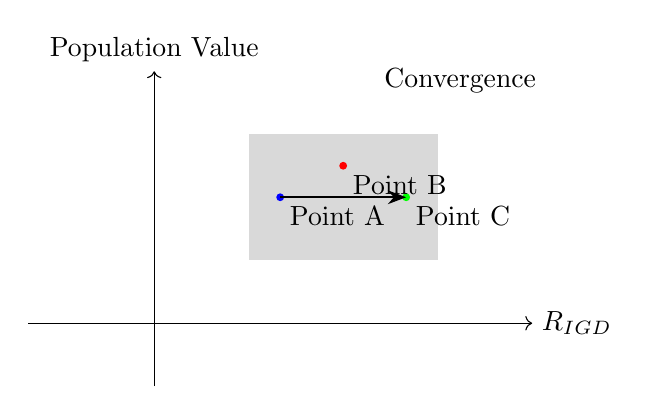
\begin{tikzpicture}[scale=0.8]

        % Axis for Part (a)
        \draw[->] (-2, 0) -- (6, 0) node[right] {$R_{IGD}$};
        \draw[->] (0, -1) -- (0, 4) node[above] {Population Value};
        
        % Shaded Area
        \fill[gray!30] (1.5, 1) rectangle (4.5, 3);
        
        % Points
        \node[circle, fill=blue, inner sep=1pt] at (2, 2) {};
        \node[circle, fill=red, inner sep=1pt] at (3, 2.5) {};
        \node[circle, fill=green, inner sep=1pt] at (4, 2) {};

        % Labels
        \node at (2, 2) [below right] {Point A};
        \node at (3, 2.5) [below right] {Point B};
        \node at (4, 2) [below right] {Point C};

        % Arrow indicating convergence
        \draw[-Stealth, thick] (2, 2) -- (4, 2);

        % Text annotation
        \node at (3.5, 3.5) [above right] {Convergence};

    \end{tikzpicture}
    \quad
    \begin{tikzpicture}[scale=0.8]

        % Axis for Part (b)
        \draw[->] (-2, 0) -- (6, 0) node[right] {$\gamma$};
        \draw[->] (0, -1) -- (0, 4) node[above] {$Variance$};
        
        % Points
        \node[circle, fill=blue, inner sep=1pt] at (2, 3) {};
        \node[circle, fill=red, inner sep=1pt] at (3,